
\section{Interpretando o Modelo e Análise de Influência das Features} 
\label{sec:avaliacao}

Este capítulo descreve o processo de interpretação dos resultados obtidos pelo modelo selecionado para a detecção de malwares. A interpretabilidade é um componente crítico em segurança cibernética, pois permite não apenas a classificação, mas a compreensão dos comportamentos que levam o modelo a identificar uma ameaça.

\subsection{Seleção e Treinamento do Modelo} \label{subsec:treinamento}

Com base em experimentos prévios, o modelo de \textbf{Regressão Logística} foi o escolhido para a análise final. Esta decisão fundamentou-se no fato de o modelo apresentar resultados de acurácia próximos aos do Random Forest, porém com um desempenho de processamento e eficiência computacional consideravelmente superiores. O treinamento foi realizado utilizando os seguintes hiperparâmetros otimizados:

\begin{itemize}
    \item Penalidade: $L1$ Lasso (Least Absolute Shrinkage and Selection Operator);
    \item Parâmetro de Regularização ($C$): $1.0$;
    \item Solucionador: \textit{saga};
    \item Máximo de iterações: $1000$.
\end{itemize}

\subsection{Cálculo Nativo de Importância (Coeficientes)} \label{subsec:calcnativo}

A Regressão Logística, por ser um modelo linear, permite uma interpretação direta através de seus coeficientes \cite{hosmer2013applied}. Cada variável de entrada (feature) recebe um peso que representa sua contribuição para o log-odds da classe alvo.

\begin{figure}[htbp]
    \centering
    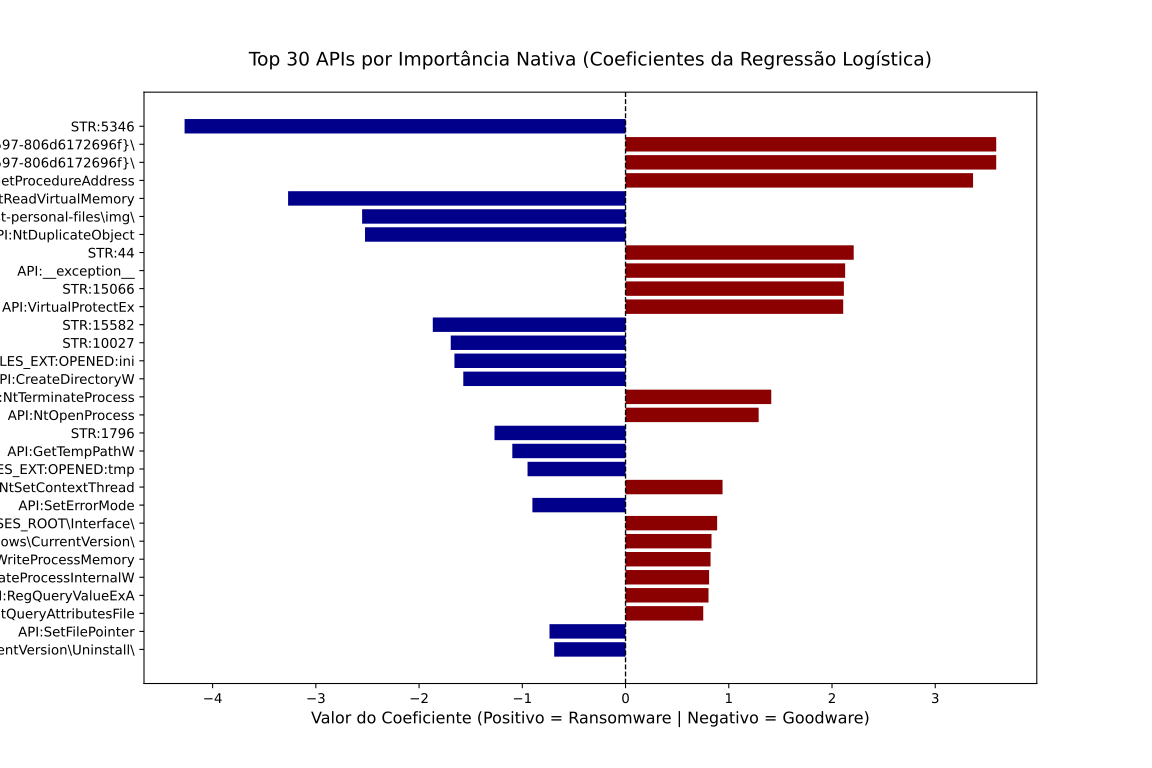
\includegraphics[width=0.8\textwidth]{images/calcnativo_regressao.png}
    \caption{Grafico do Calculo Nativo do modelo Logistic Regression em seus melhores parametros.}
    \label{fig:calcnativo-regressao}
\end{figure}

A Figura ~\ref{fig:calcnativo-regressao} apresenta o \textit{Top 30 APIs por Importância Nativa}. No gráfico:
\begin{itemize}
    \item \textbf{Coeficientes Positivos (Vermelho):} Indicam que a presença ou alta frequência da API aumenta a probabilidade de a amostra ser classificada como \textit{Ransomware}. Destacam-se APIs relacionadas a manipulação de strings e acesso a registros.
    \item \textbf{Coeficientes Negativos (Azul):} Indicam uma associação com \textit{Goodware}. A API \texttt{STR:5346} e \texttt{API:NtReadVirtualMemory} apresentam os maiores pesos negativos, sugerindo que são características predominantes em softwares legítimos no dataset analisado.
\end{itemize}

\subsection{Análise de Explicabilidade com SHAP} \label{subsec:shap}

Para aprofundar a compreensão sobre a influência das features, utilizamos o framework SHAP (\textit{SHapley Additive exPlanations}), fundamentado na teoria dos jogos cooperativos \cite{lundberg2017unified}. O SHAP oferece uma visão mais granular do que os coeficientes globais, permitindo observar o impacto de cada feature em cada predição individual.

\subsubsection{Beeswarm Plot} \label{subsubsec:beeswarm}

O gráfico \textit{Beeswarm} (Figura ~\ref{fig:beeswarm}) fornece uma visão geral do impacto das top 30 APIs no modelo.

\begin{figure}[htbp]
    \centering
    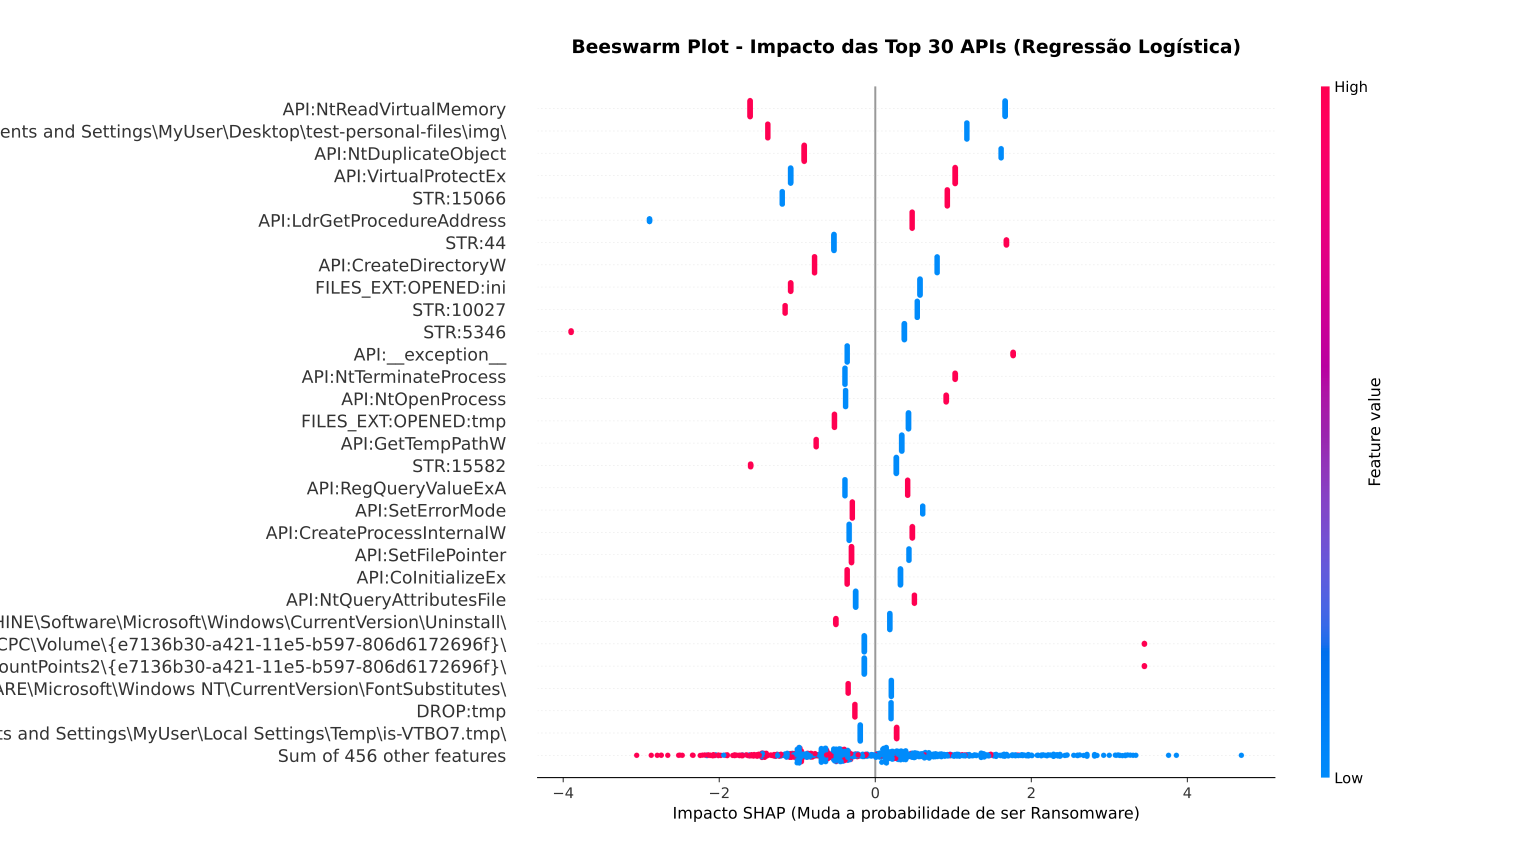
\includegraphics[width=0.8\textwidth]{images/shap_lregression_beeswarm.png}
    \caption{Grafico SHAP Beeswarm com o modelo Logistic Regression em seus melhores parametros.}
    \label{fig:beeswarm}
\end{figure}

\begin{itemize}
    \item O eixo horizontal representa o \textbf{Impacto SHAP}: valores à direita aumentam a probabilidade de \textit{Ransomware}, enquanto à esquerda diminuem.
    \item A cor indica o valor da feature (Vermelho para alto, Azul para baixo). 
    \item Observa-se que para a API \texttt{NtReadVirtualMemory}, valores baixos (azul) têm um impacto negativo forte, corroborando o gráfico de coeficientes nativos, enquanto para outras APIs, a dispersão dos pontos revela comportamentos não lineares capturados pelo modelo.
\end{itemize}

\subsubsection{Decision Plot} \label{subsubsec:decisionplot}

O grafico \textit{Decision Plot} Figura ~\ref{fig:bdecision} ilustra o caminho de decisão para 50 amostras específicas.

\begin{figure}[htbp]
    \centering
    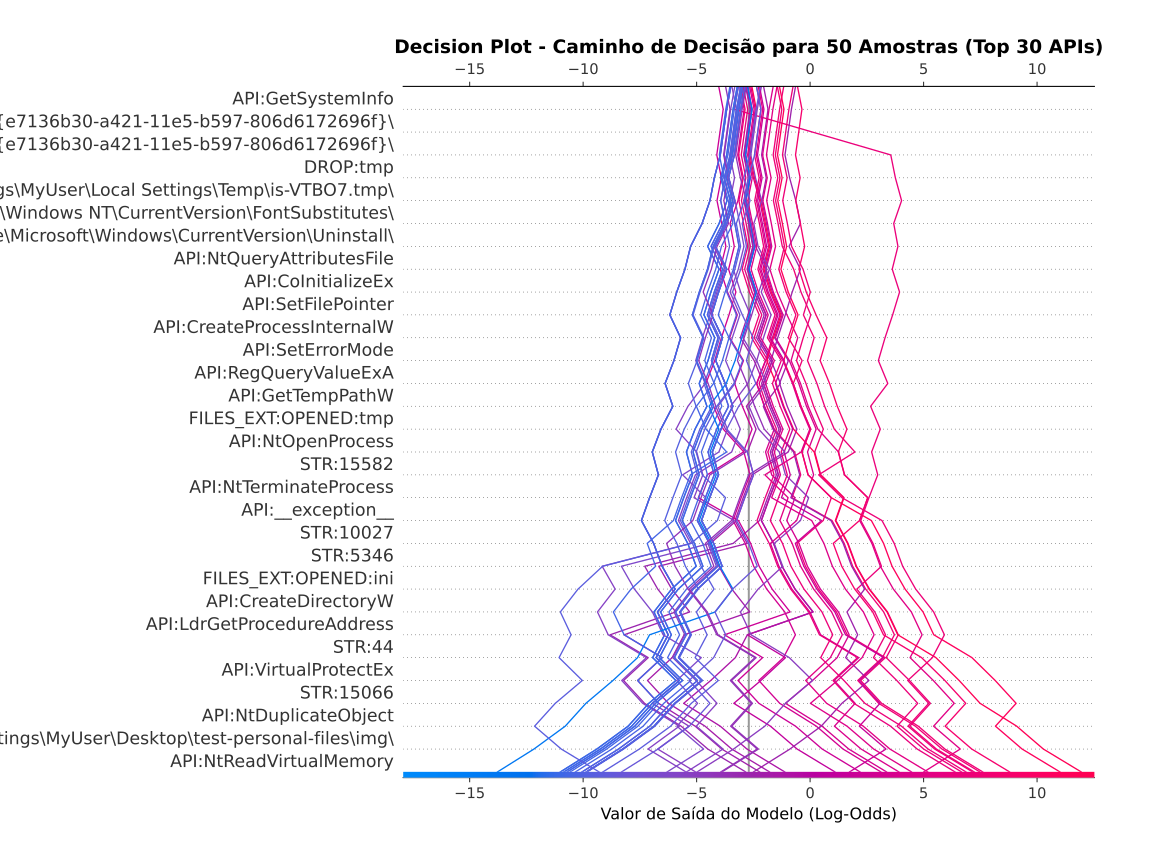
\includegraphics[width=0.8\textwidth]{images/shap_lregression_bdecision.png}
    \caption{Grafico SHAP Decision Plot com o modelo Logistic Regression em seus melhores parametros.}
    \label{fig:bdecision}
\end{figure}

\begin{itemize}
    \item O gráfico mostra como as predições individuais evoluem a partir de um valor base (valor médio esperado) conforme cada API é considerada.
    \item As linhas que convergem para a direita (em rosa) representam amostras com alta probabilidade de serem maliciosas, enquanto as que tendem para a esquerda (em azul) são classificadas como benignas.
    \item Este gráfico é essencial para identificar quais combinações de APIs são determinantes para a classificação final do modelo em casos específicos de \textit{log-odds}.
\end{itemize}